\subsubsection{GPS}

El GPS (\textit{Global Positioning System}) es una tecnología de navegación por satélite que permite determinar la ubicación geográfica exacta de un objeto o dispositivo en cualquier parte del mundo. El sistema fue desarrollado por el Departamento de Defensa de los Estados Unidos \cite{gps} y está compuesto por una red de satélites que transmiten señales de tiempo y posición generalmente en la banda de frecuencia L1 1.57542 GHz para usos civiles. Los dispositivos con receptores GPS pueden calcular su posición en la Tierra midiendo el tiempo que tarda la señal en viajar desde los satélites. \\


El GPS utiliza una técnica llamada trilateración para determinar la posición de un dispositivo. Para calcular su ubicación, el receptor GPS necesita recibir señales de al menos cuatro satélites. A partir de estas señales, el receptor puede calcular la distancia a cada satélite y determinar con precisión su posición en coordenadas geográficas (latitud, longitud y altitud). El GPS utiliza cuatro satélites en lugar de tres para calcular no solo la ubicación en tres dimensiones, sino también para corregir errores en el reloj del receptor y obtener mayor precisión. En la figura \ref{fig:gps} se visualiza cómo un receptor recibe señales de 4 satélites lo que le permite determinar su ubicación. \\

\begin{figure}[H]
    \centering
    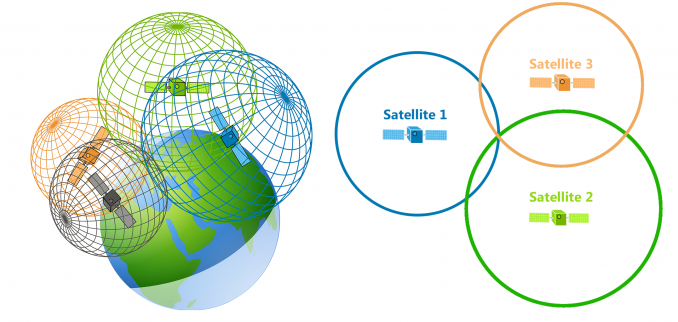
\includegraphics[width = 0.7 \linewidth]{img/gps.png}
    \caption{Trilateración utilizada en GPS \cite{gps_img}}
    \label{fig:gps}
\end{figure}



En los sistemas embebidos, los módulos GPS se utilizan ampliamente para aplicaciones que requieren posicionamiento y geolocalización. Estos módulos son pequeños, de bajo consumo de energía y fáciles de integrar en una amplia variedad de dispositivos y proyectos. Algunas aplicaciones comunes en sistemas embebidos incluyen:

\begin{itemize}
    \item \textbf{Monitoreo de vehículos}: El GPS es utilizado para rastrear vehículos en tiempo real, facilitando sistemas de logística, transporte público y servicios de emergencia.

    \item \textbf{Agricultura de precisión}: Equipos agrícolas con GPS pueden optimizar la siembra, el riego y la cosecha mediante la geolocalización precisa.

    \item \textbf{Dispositivos IoT}: Muchos dispositivos conectados a internet, como drones, sensores o sistemas de automatización, utilizan GPS para la recolección de datos de ubicación.

    \item \textbf{Navegación y mapeo}: Desde sistemas de navegación portátiles hasta drones y robots autónomos, el GPS permite trazar rutas y moverse eficientemente por entornos dinámicos.
\end{itemize}


La utilización de GPS provee una alta precisión que varía desde los pocos metros hasta los centímetros (dependiendo de las condiciones y el equipo). También tiene la ventaja de contar con una cobertura global lo que permite una solución de geolocalización sin necesidad de infraestructura adicional. Además, los módulos GPS para sistemas embebidos están diseñados para ser eficientes energéticamente, lo que los hace ideales para dispositivos portátiles o alimentados por baterías. \\ 

En resumen, la tecnología GPS ha revolucionado la capacidad de los sistemas embebidos para obtener y procesar datos de ubicación de manera eficiente y precisa. Su integración en dispositivos y aplicaciones es clave para una variedad de sectores, como la logística, la agricultura y el IoT, proporcionando soluciones versátiles y de bajo consumo para necesidades de geolocalización. La combinación de su cobertura global y su capacidad de adaptación lo convierte en una herramienta fundamental en el diseño de sistemas embebidos modernos.